\documentclass[12pt,a4paper]{article}
\synctex=1
\usepackage[utf8]{inputenc}
\usepackage[margin=1cm]{geometry}
\usepackage{graphicx}
%\usepackage{verbatim}
\usepackage{amsmath}
\usepackage{amsfonts}
\usepackage{amssymb}
\usepackage{listings}
\usepackage{enumitem}
\usepackage{textcomp}
\usepackage{courier}
\usepackage{libertine}
\usepackage{pgfornament}
\usepackage{eso-pic}
\usepackage[hangul]{kotex}
\linespread{1.3}

\title{
	\centering
	\pgfornament[width=12cm,color=teal]{84}\\
	\vspace{1cm}
	\fontsize{50}{50} \selectfont {정보통신 수학 및 실습\\Homework}\\
		\pgfornament[width=12cm,color=teal]{88}\\
	\vfill}
\author{
	\LARGE
	\begin{tabular}{rl}
		\hline
		학번 : & 2016110056\\ 
		학과 : & 불교학부 \\
		이름 : & 박승원\\
		날짜 : & \today\\
		\hline
	\end{tabular}\vspace{2cm}
	\\
\includegraphics[width=0.5\textwidth]{logo.jpg}
	}
\date{}


\begin{document}
\maketitle
\pagenumbering{gobble}
\noindent
\lstset{language=matlab, columns=flexible, tabsize=4, frame=shadowbox, showstringspaces=false, breaklines=true, upquote=true, basicstyle=\normalsize}

\renewcommand{\thesubsubsection}{\alph{subsubsection})}
\renewcommand{\thesubsection}{\arabic{subsection}.}
\newpage

\section*{Chapter 11 Homework}
\subsection{Find the Fourier series of the following functions. } 
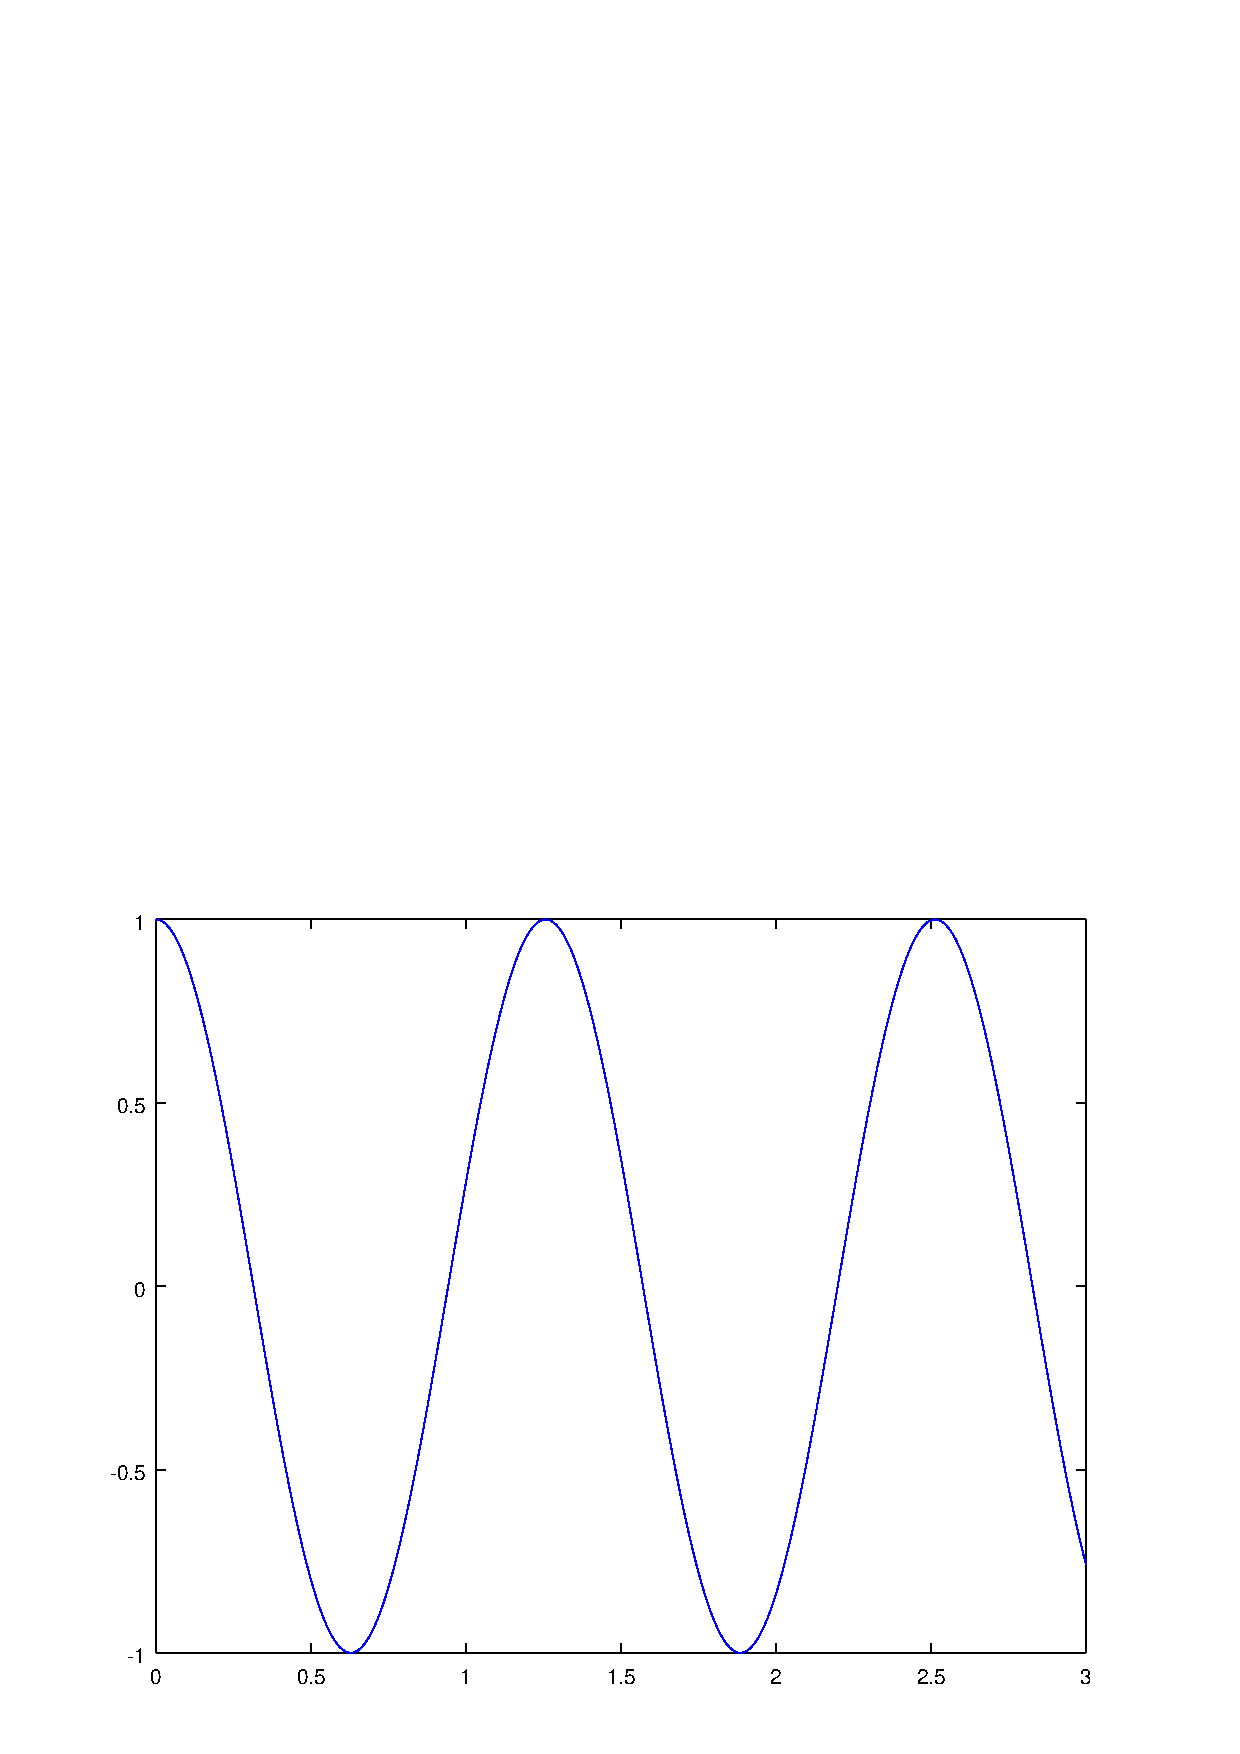
\includegraphics[width=0.8\textwidth]{a.png}

\begin{gather*}
\int_{-\infty}^{\infty} f(t)e^{-j2\pi ft}dt
=100\int_{-1}^{1}e^{-j2\pi ft}dt
=100\left[\frac{e^{-j2\pi ft}}{-j2\pi f}\right]_{-1}^1
=100(\frac{e^{-j2\pi f}}{-j2\pi f}-\frac{e^{j2\pi f}}{-j2\pi f})
=100(\frac{e^{j2\pi f}-e^{-j2\pi f}}{j2\pi f})\\
=100(\frac{2j\sin 2\pi f}{j2\pi f})
=\frac{200\sin 2\pi f}{2\pi f}\\
\end{gather*}
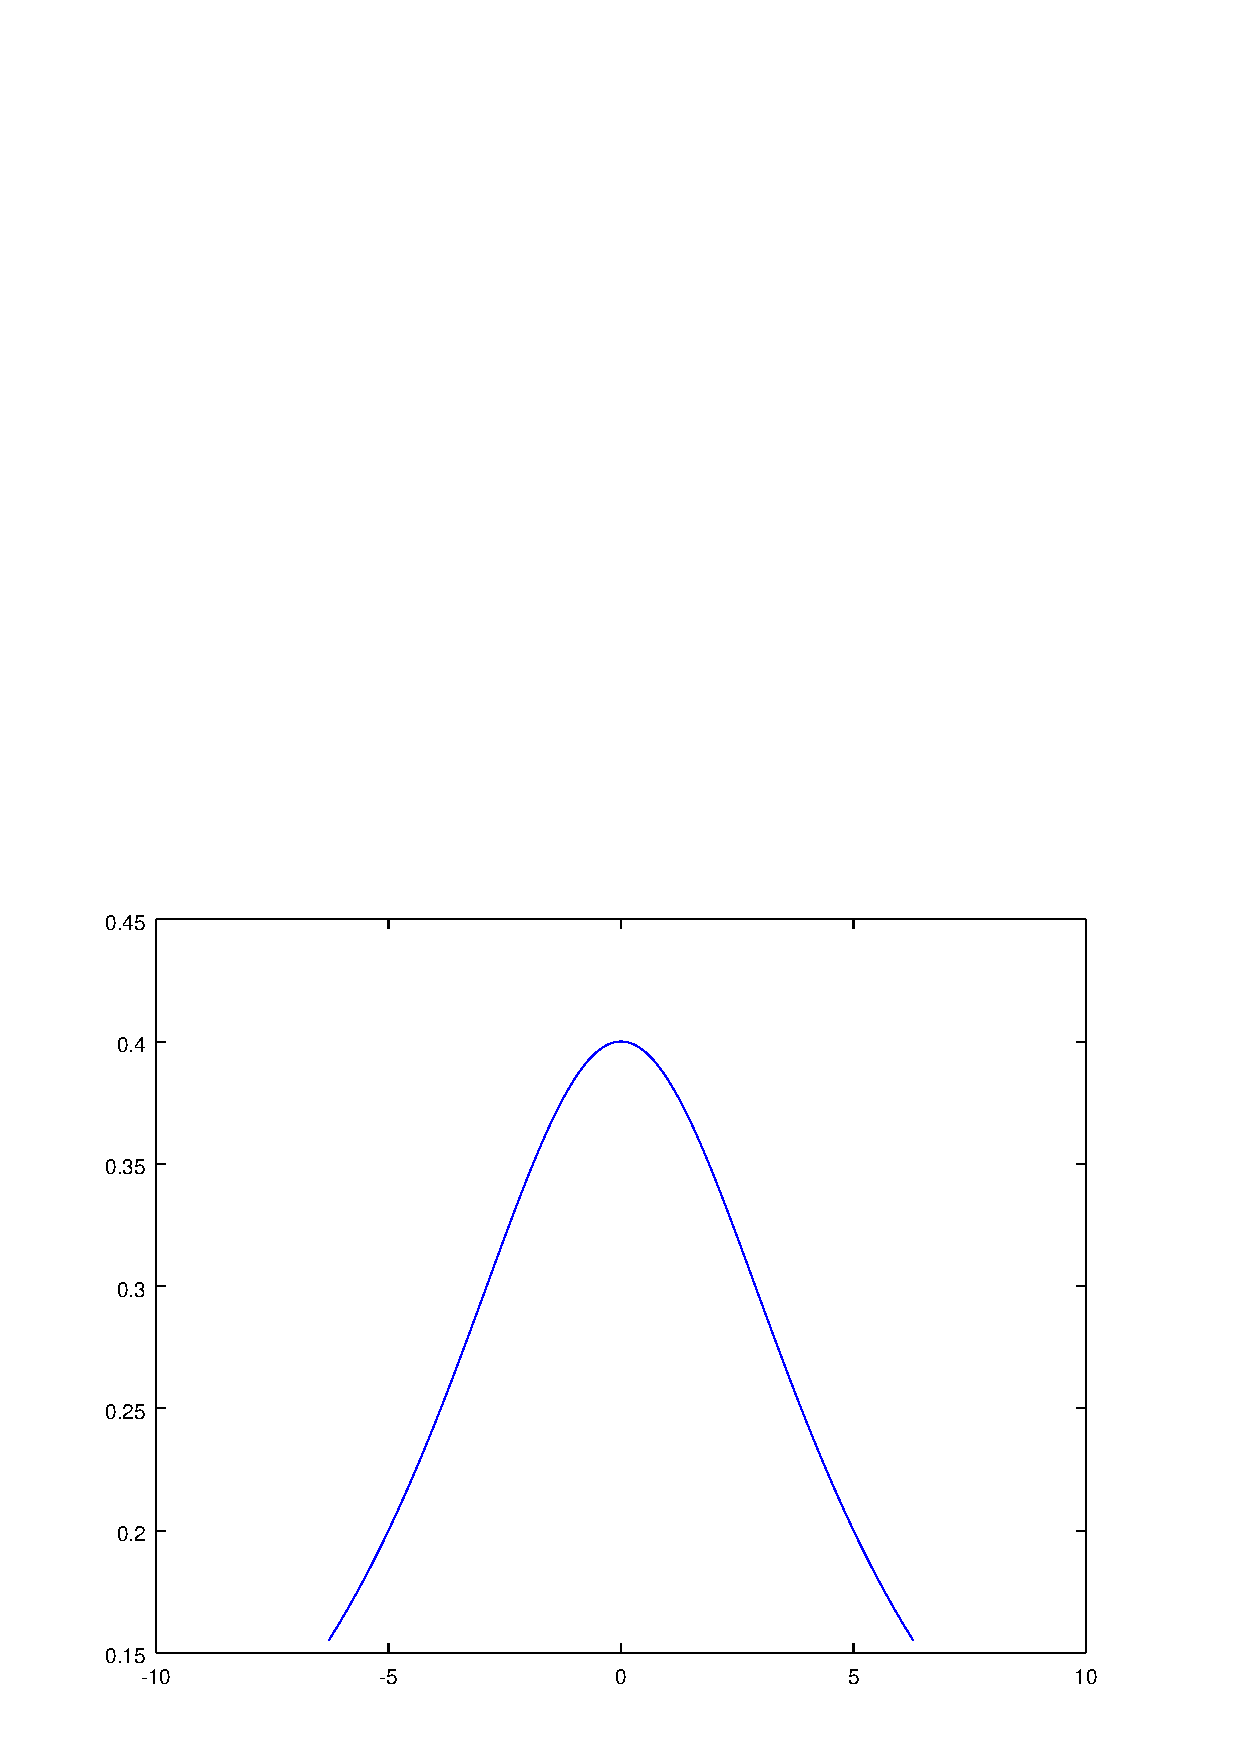
\includegraphics[width=0.8\textwidth]{3.png}

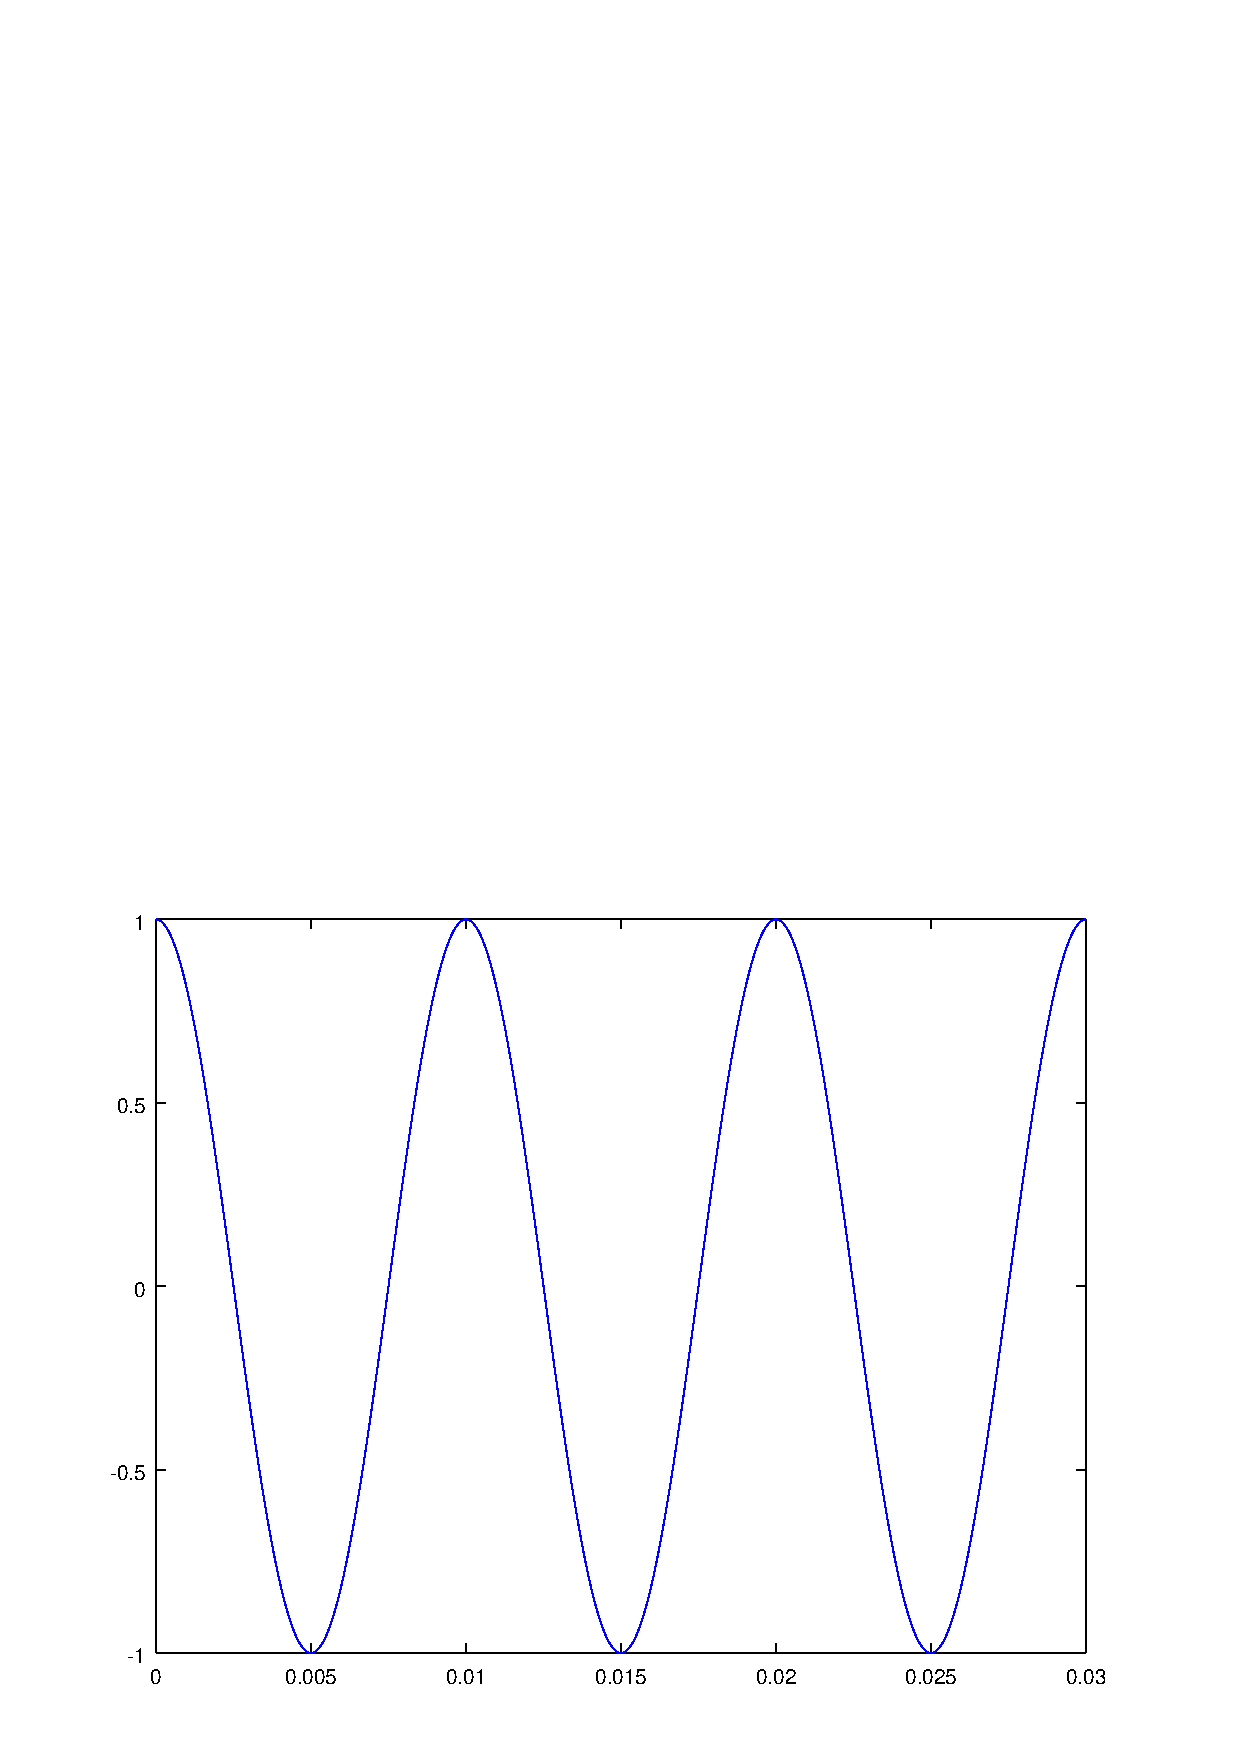
\includegraphics[width=0.8\textwidth]{b.png}
\begin{gather*}
\int_{-\infty}^{\infty}f(t)e^{-2j\pi ft}dt
=\int_{-1}^{0}(x+1)e^{-2j\pi ft}dt + \int_{0}^{1}(-x+1)e^{-2j\pi ft}dt\\
=\int_{-1}^{0}xe^{-j2\pi ft}dt - \int_{0}^{1}xe^{-j2\pi ft}dt + \int_{-1}^{1}e^{-j2\pi ft}dt\\
\because \int uv' = uv - \int u'v\\
=\left[x\frac{e^{-j2\pi ft}}{-j2\pi f}\right]_{-1}^0 - \int_{-1}^{0}\frac{e^{-j2\pi ft}}{-j2\pi f}dt
-\left[x\frac{e^{-j2\pi ft}}{-j2\pi f}\right]_{0}^1 + \int_{0}^{1}\frac{e^{-j2\pi ft}}{-j2\pi f}dt
+\left[\frac{e^{-j2\pi ft}}{-j2\pi f}\right]_{-1}^1\\
=-\int_{-1}^{0}\frac{e^{-j2\pi ft}}{-j2\pi f}dt  +
\int_{0}^{1}\frac{e^{-j2\pi ft}}{-j2\pi f}dt
=-\left[\frac{e^{-j2\pi ft}}{-4\pi^2f^2}\right]_{-1}^0 + 
\left[\frac{e^{-j2\pi ft}}{-4\pi^2 f^2}\right]_0^1
=\frac{e^{-j2\pi f}}{4\pi^2f^2} + \frac{e^{-j2\pi f}}{4\pi^2 f^2}
=\frac{\cos(2\pi f)}{2\pi^2 f^2}
\end{gather*}
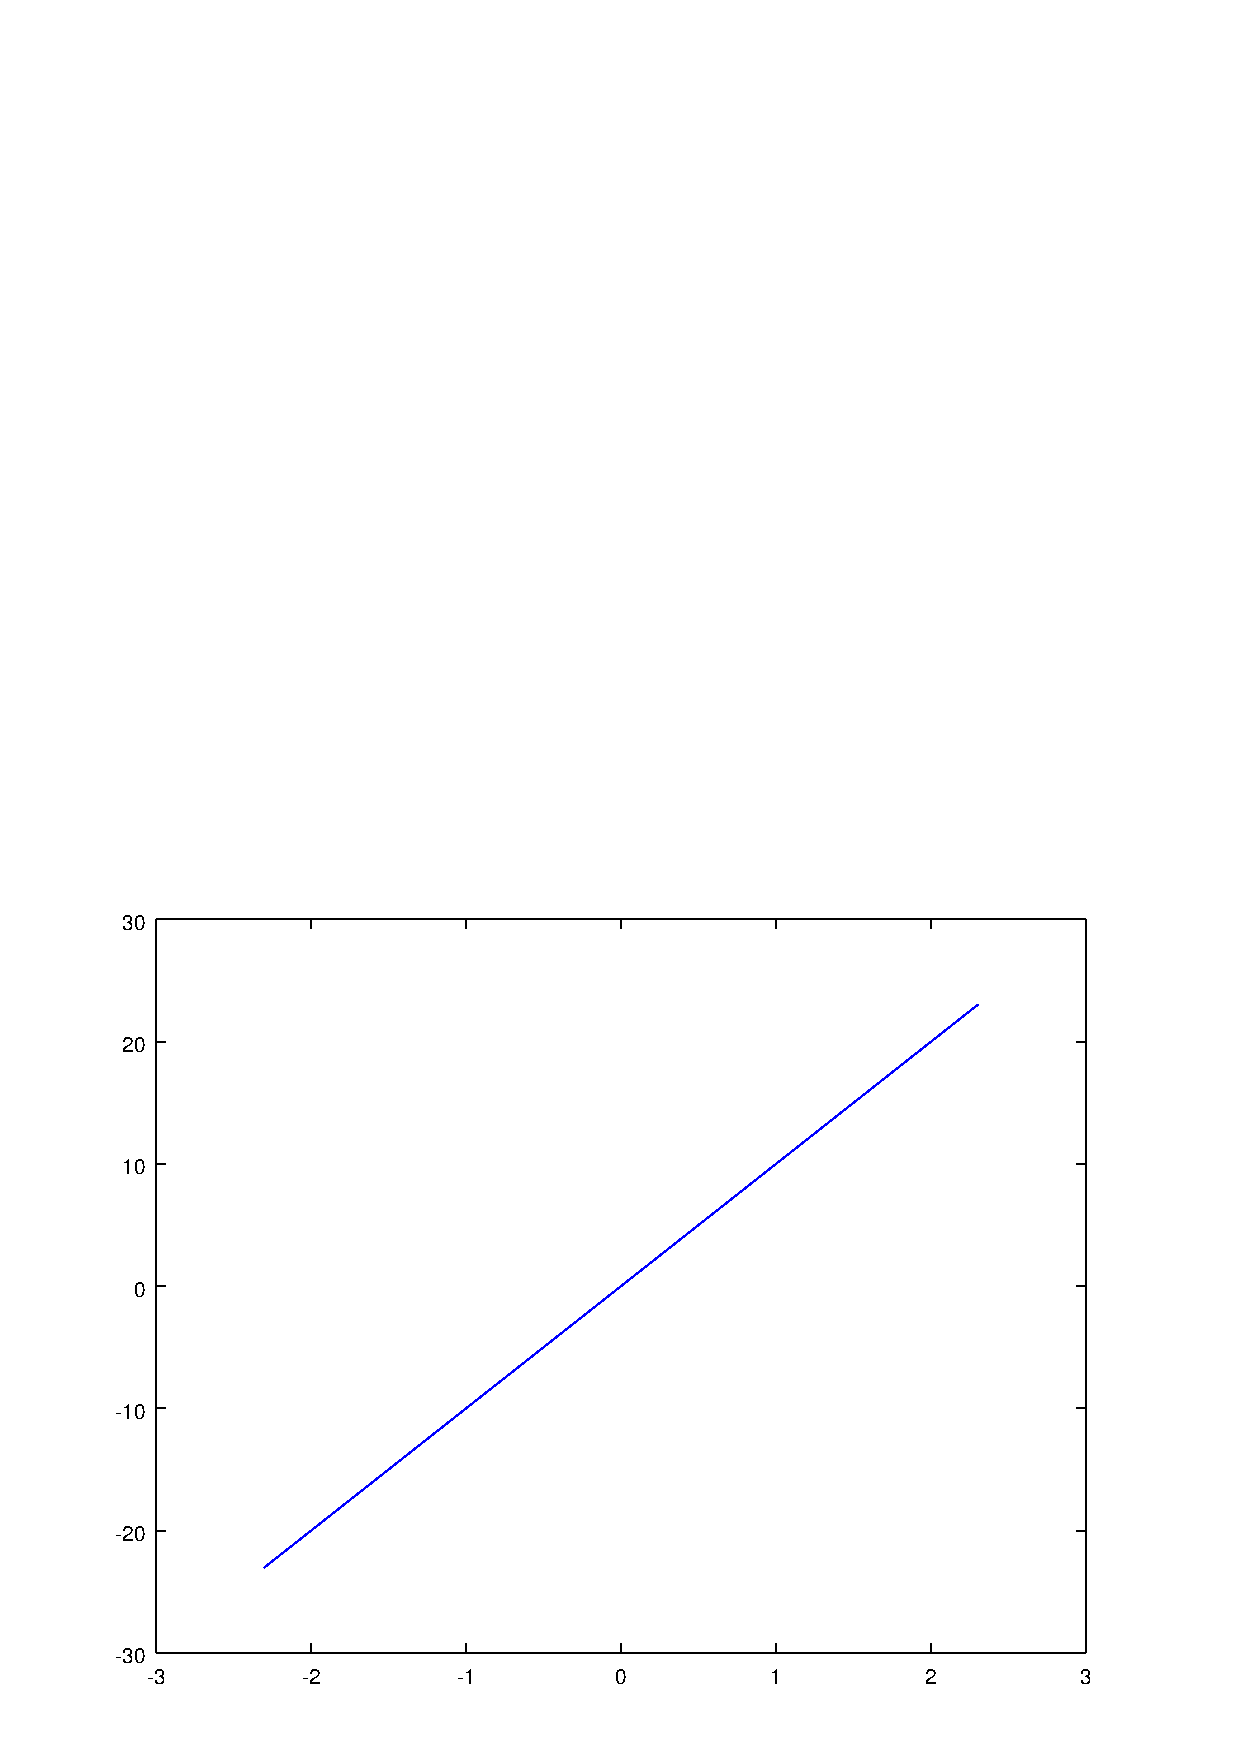
\includegraphics[width=0.8\textwidth]{4.png}

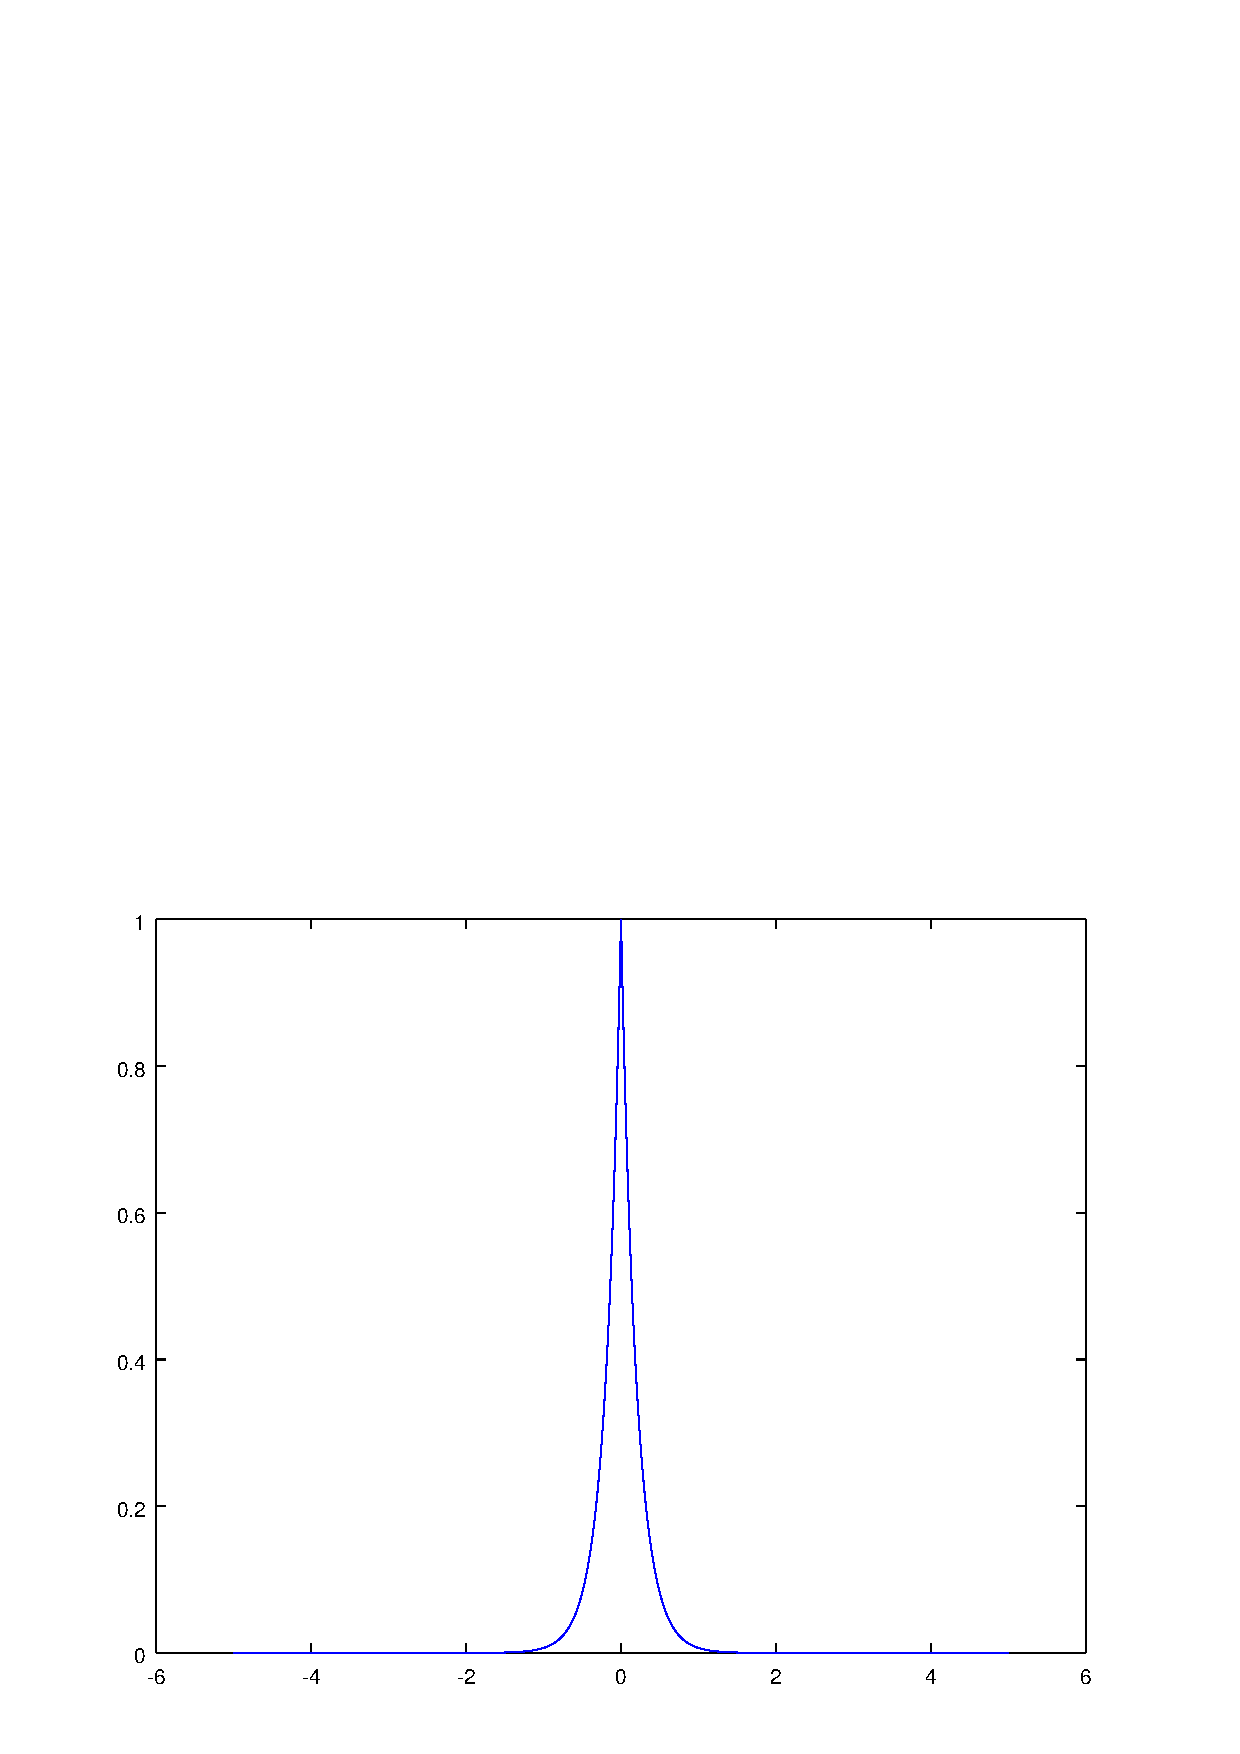
\includegraphics[width=0.8\textwidth]{2.png}
\begin{gather*}
\int_{-\infty}^{\infty}f(t)e^{-j2\pi ft}dt
=\int_{-\infty}^{0}e^{7t}e^{-j2\pi ft}dt + \int_{0}^{\infty}e^{-7t}e^{-j2\pi ft}dt
=\left[\frac{e^{(7-j2\pi f)t}}{7-j2\pi f}\right]_{-\infty}^0
+\left[\frac{e^{(-7-2j\pi f)t}}{-7-j2\pi f}\right]_0^{\infty}\\
=-\frac{1}{7-j2\pi f} - \frac{1}{7+j2\pi f} = -\frac{14}{49+4\pi^2 f^2}
\end{gather*} 
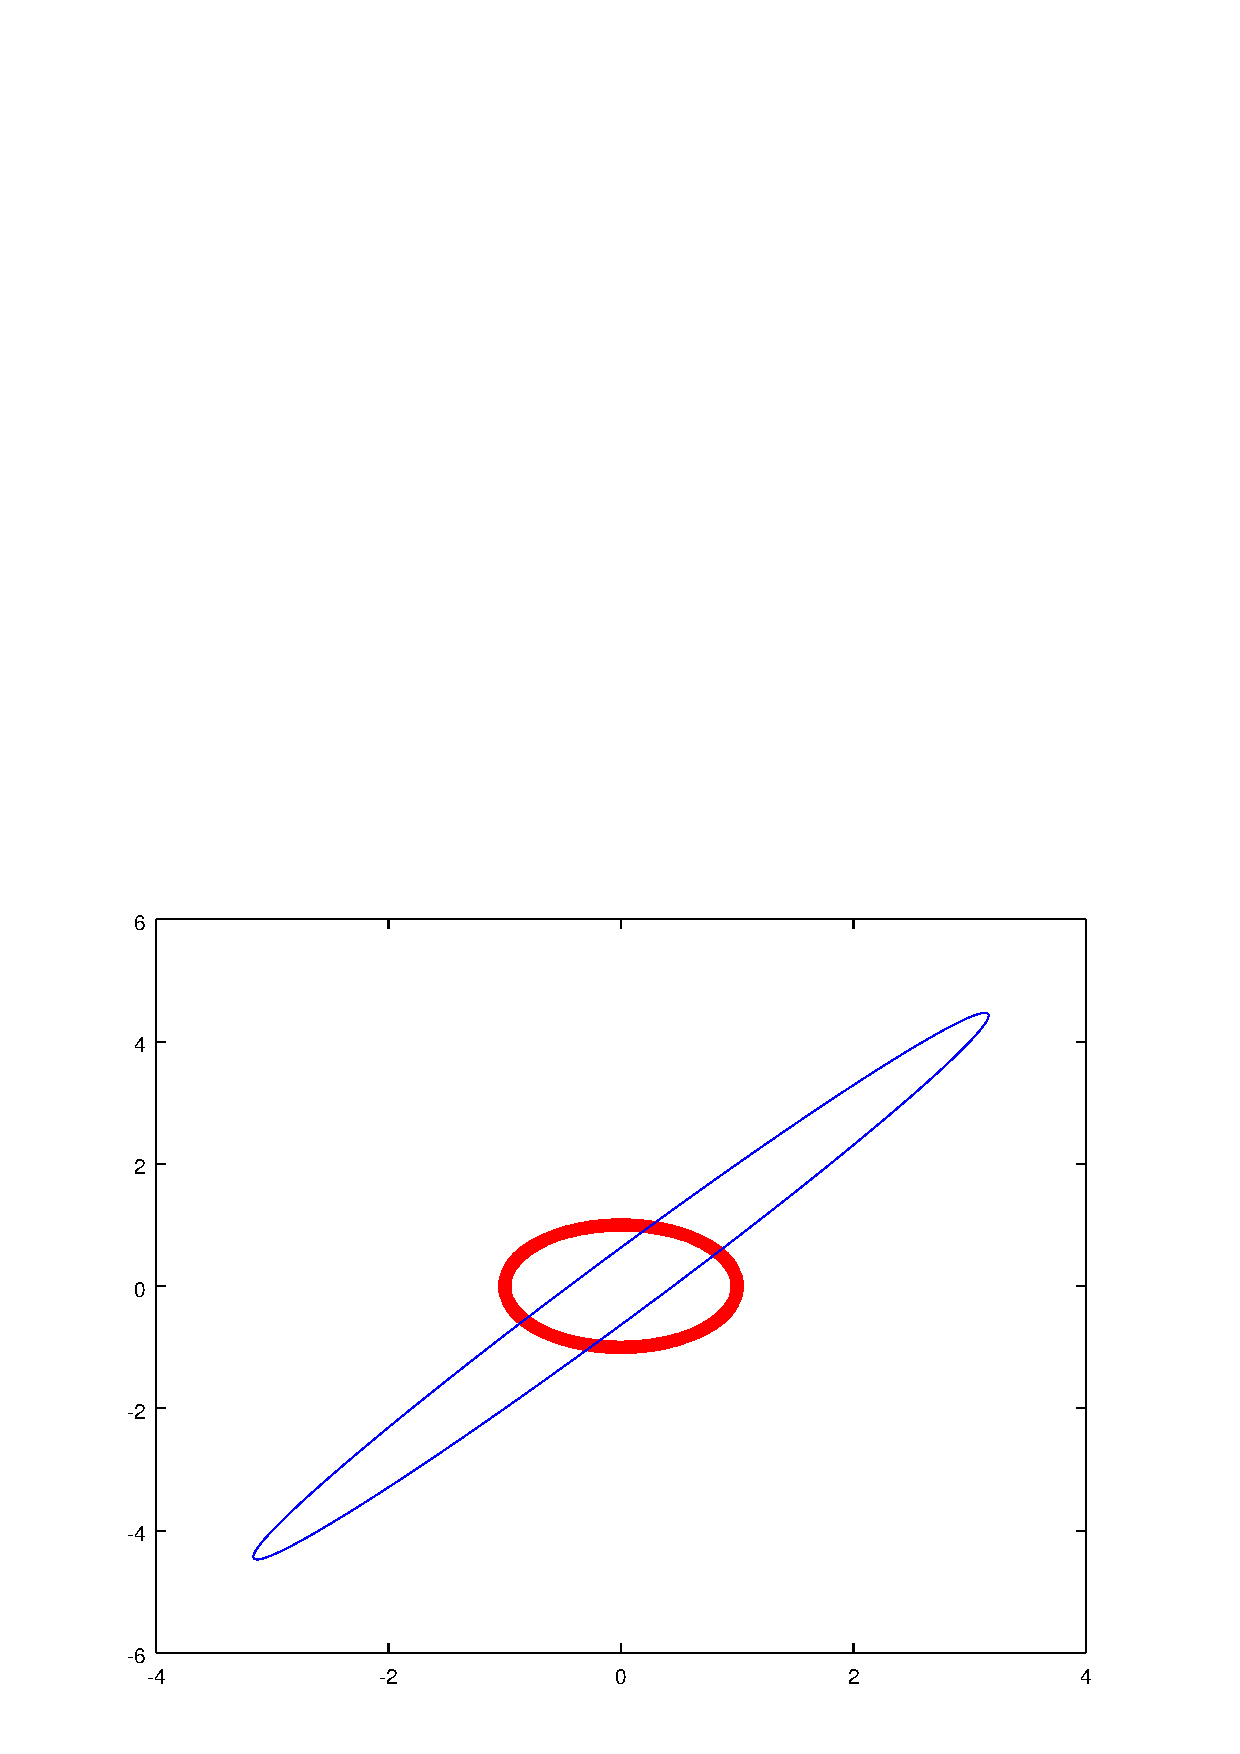
\includegraphics[width=0.8\textwidth]{5.png}
\end{document}
